\subsection{Welten}
\mysubsubsection{Lydia Friedrich}{Gebirgswelt}

\begin{figure}[!htbp]%[htbp]
	\centering
		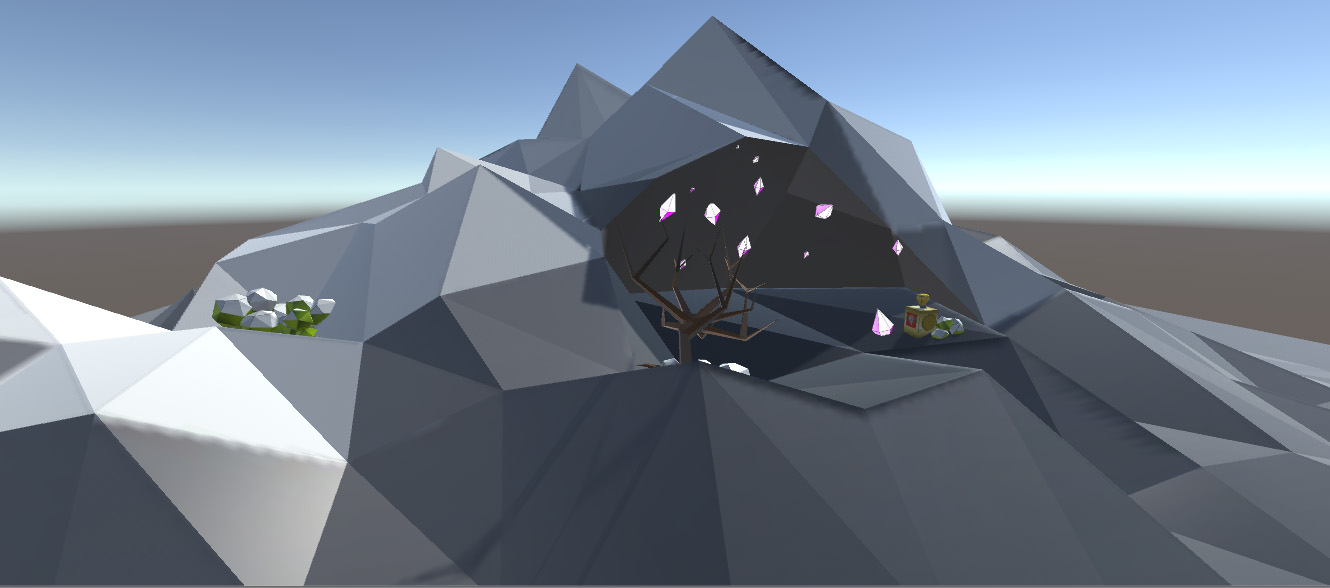
\includegraphics[width=1.0\textwidth]{images/Gebirge}
	\caption{Screenshot der Gebirgslandschaft}
	\label{fig:Gebirge}
\end{figure}

Die Gebirgswelt ist die einzige Welt die der Nutzer zu Beginn des Spiels ansteuern und erkunden kann. Die leuchtenden Kristalle, innerhalb der Berghöhle, erzeugen in der Dunkelheit eine mysteriöse und wahrscheinlich aufregende Stimmung. So bald der Würfel mit Licht gefüllt ist, nimmt der Spieler die Gebirgswelt erneut und sehr wahrscheinlich anders, als zuvor im Dunkeln, war. Diese Welt ist bei Tag durch einen großen Berg und den darauf lebenden Bergziegen geprägt.

\mysubsubsection{Sandra Beuck}{Dorfwelt}

\begin{figure}[!htbp]%[htbp]
	\centering
		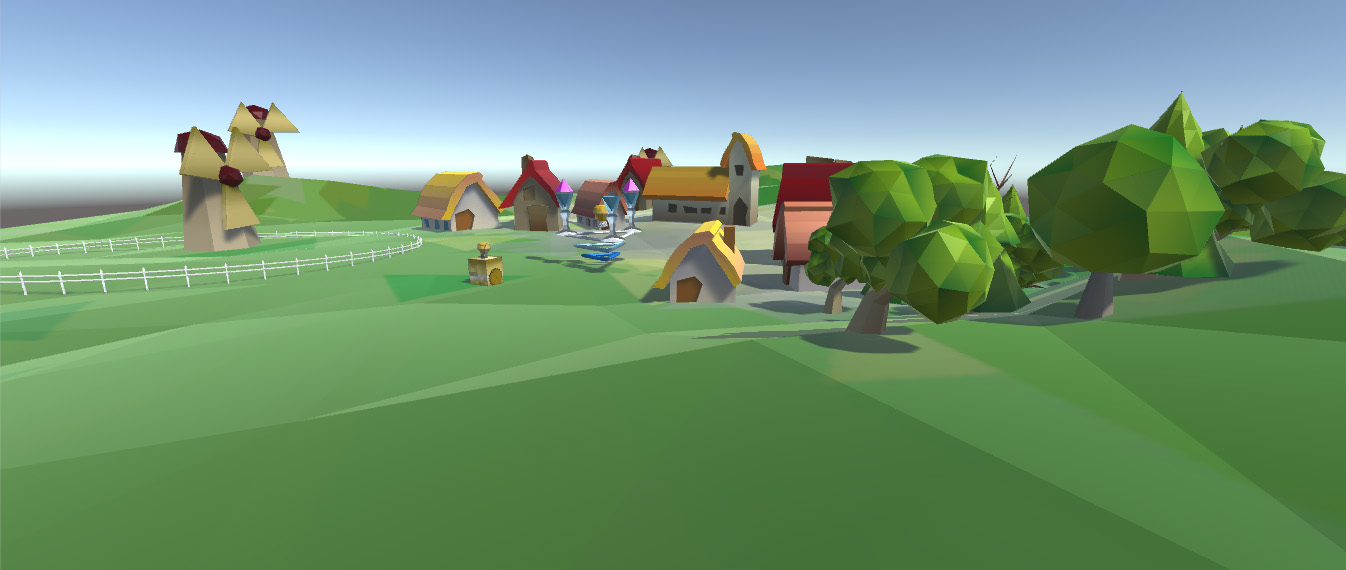
\includegraphics[width=1.0\textwidth]{images/Dorf}
	\caption{Screenshot der Dorflandschaft}
	\label{fig:Dorf}
\end{figure}

hallo

\mysubsubsection{Sandra Beuck}{Waldwelt}

\begin{figure}[!htbp]%[htbp]
	\centering
		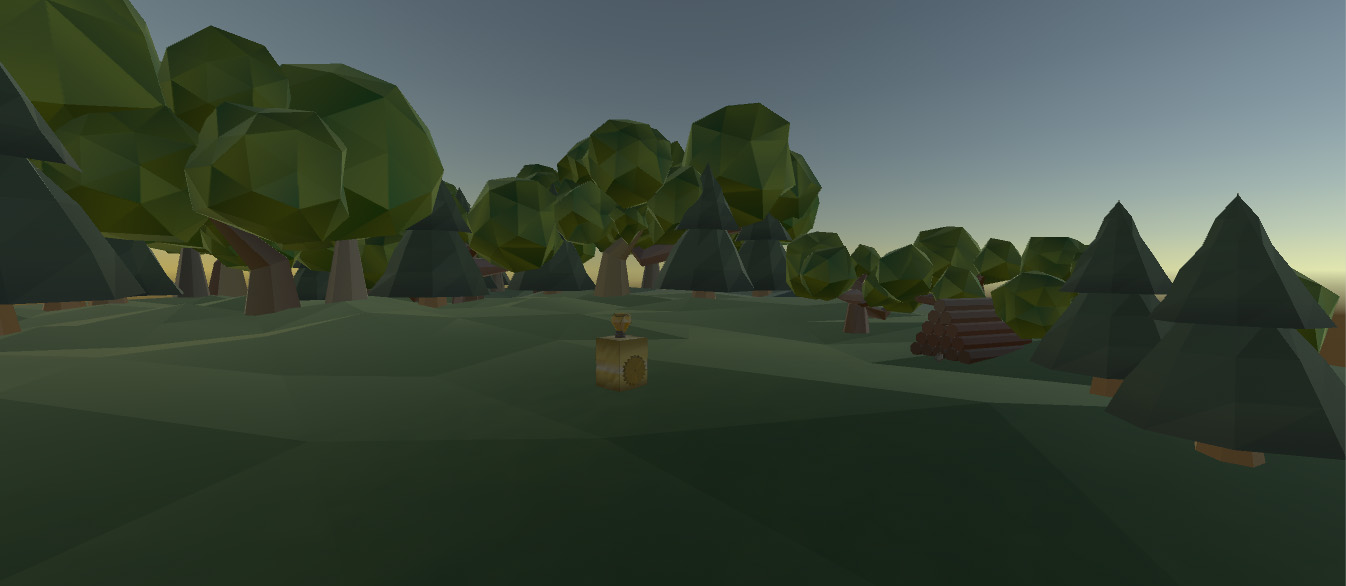
\includegraphics[width=1.0\textwidth]{images/Wald}
	\caption{Screenshot der Waldlandschaft}
	\label{fig:Wald}
\end{figure}

Diese Welt steht für das Sinnbild der Natur: der Wald. Absicht ist es, dass sich der Spieler innerhalb dieser Welt wohlfühlt. Er hat die Möglichkeit unberührte Natur zu genießen sowie Rehe in freier Wildbahn zu beobachten. Diese Welt ist durch seinen hohen Anteil an Bäumen geprägt. Der Spieler hat die Möglichkeit eines von zwei Items ein zusammeln: die Schaufel, welche an einem Holzstapel lehnt.

\mysubsubsection{Lydia Friedrich}{Wüstenwelt}

\begin{figure}[!htbp]%[htbp]
	\centering
		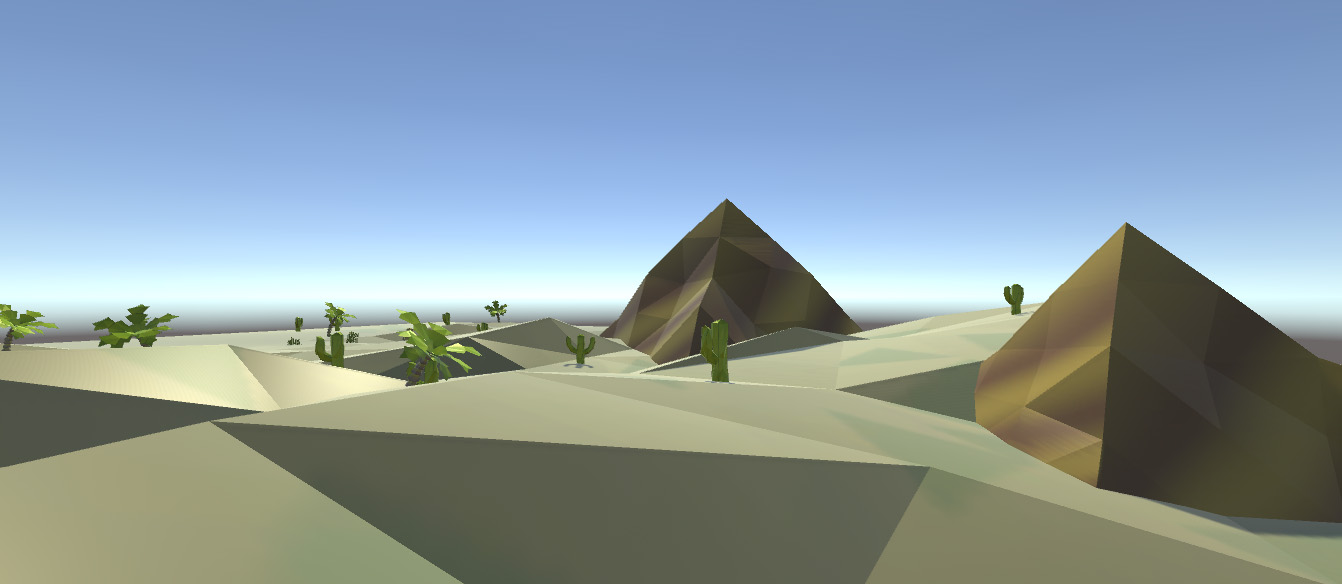
\includegraphics[width=1.0\textwidth]{images/Wueste}
	\caption{Screenshot der Wüstenlandschaft}
	\label{fig:Wueste}
\end{figure}

hallo

\mysubsubsection{Sandra Beuck}{Feuerwelt}

\begin{figure}[!htbp]%[htbp]
	\centering
		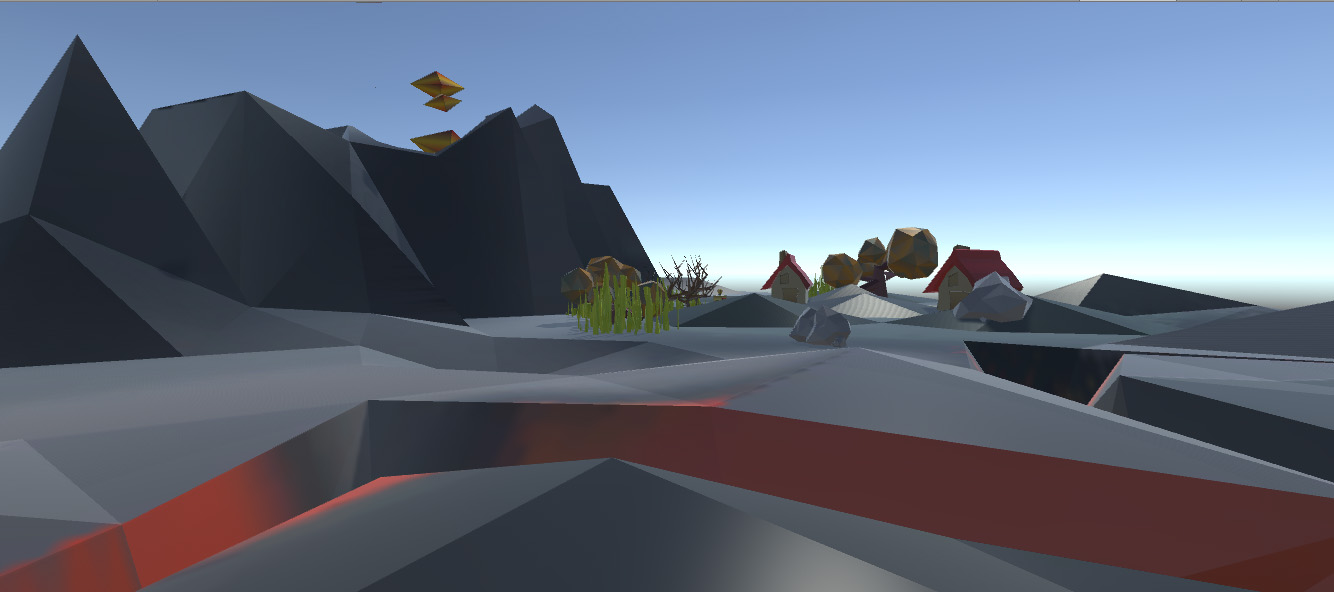
\includegraphics[width=1.0\textwidth]{images/Feuer}
	\caption{Screenshot der Feuerlandschaft}
	\label{fig:Feuer}
\end{figure}

hallo

\mysubsubsection{Lydia Friedrich}{Eiswelt}

\begin{figure}[!htbp]
	\centering
		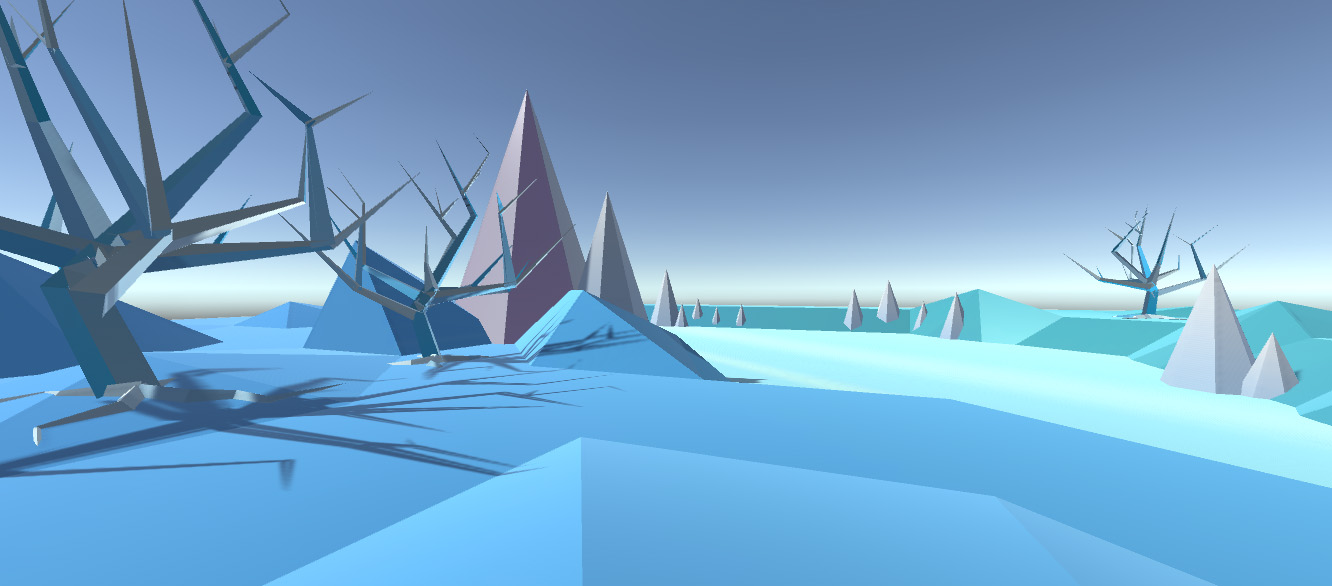
\includegraphics[width=1.0\textwidth]{images/Eis}
	\caption{Screenshot der Eislandschaft}
	\label{fig:Eis}
\end{figure}

hallo

\mysubsubsection{Lydia Friedrich}{Skybox}

%\begin{figure}[h]%[htbp]
%	\centering
%		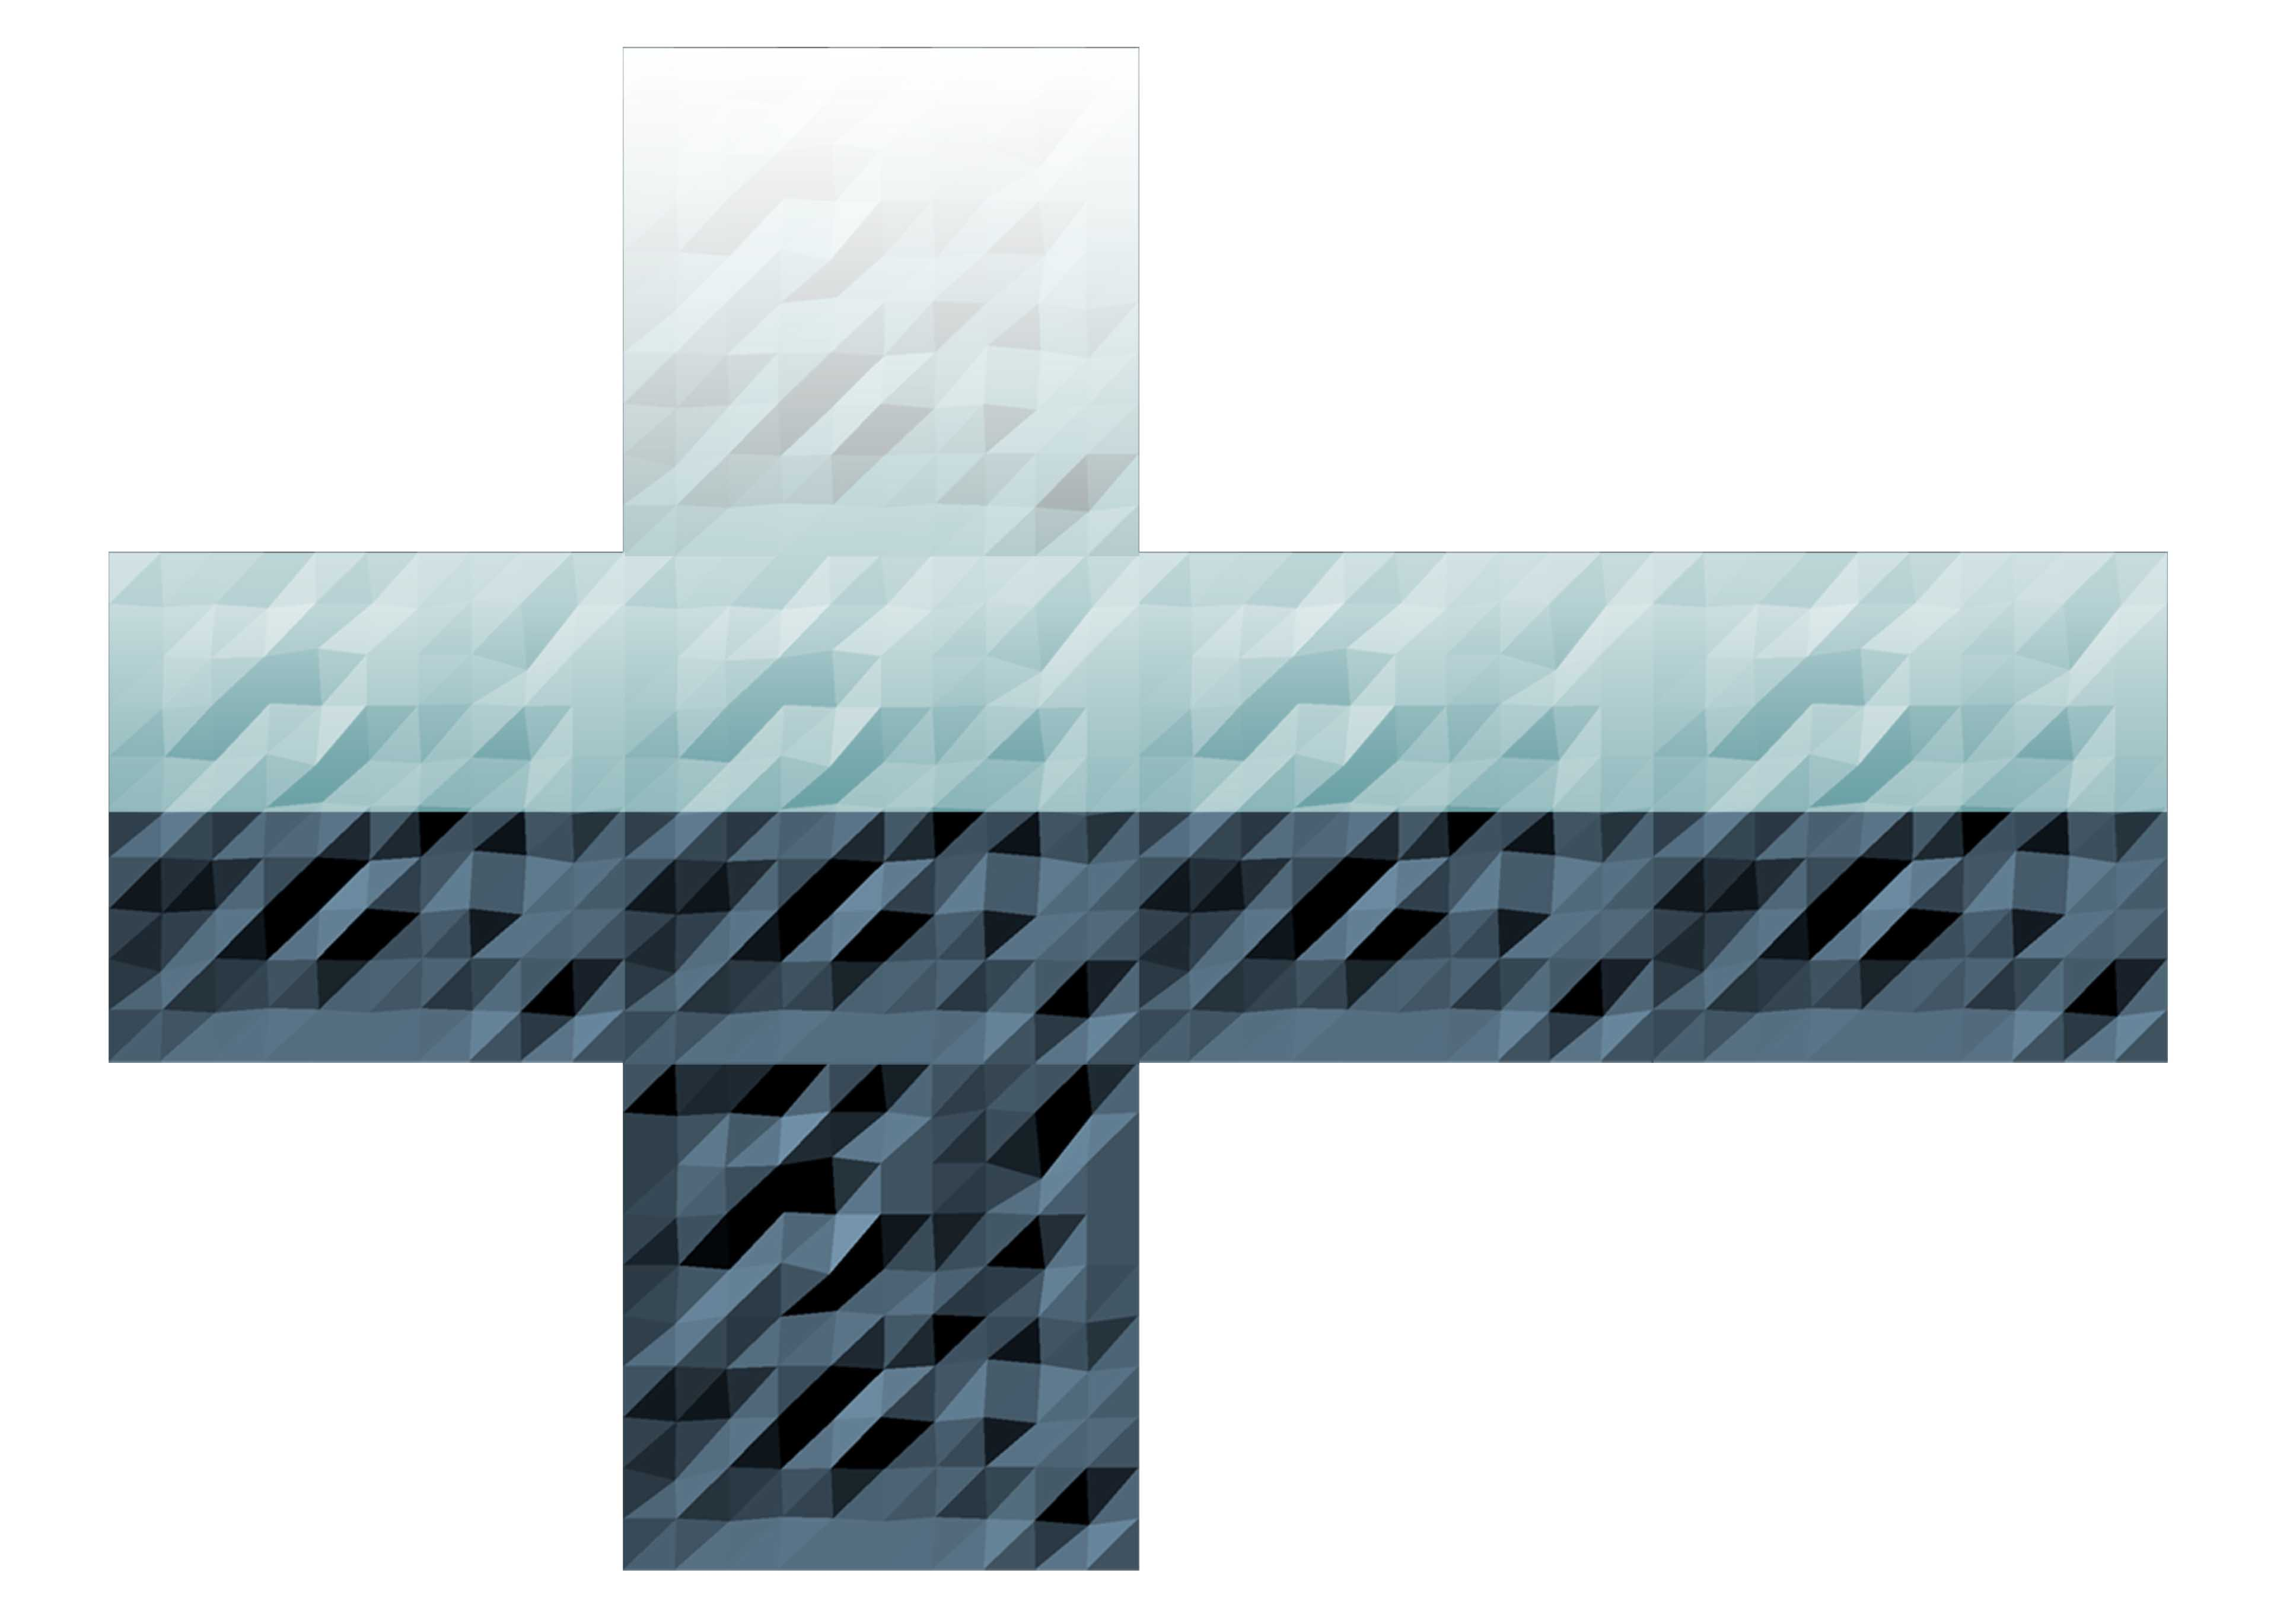
\includegraphics[width=1.0\textwidth]{images/Skybox}
%	\caption{Textur der Skybox}
%	\label{fig:Skybox}
%\end{figure}

SCREENSHOT SKYBOX

Die Skybox (siehe Abbildung \ref{fig:Skybox}) soll den charakteristischen Low Poly Stil des Spiels wiederspiegeln. Um diesen erfolgreich umzusetzen, muss ein Würfel in Cinema4D mit Hilfe des Modelling Tools bearbeitet und im Anschluss dessen Textur gebacken werden. Die Textur, welche in einer aufgeklappten Würfelform ausgegeben wird, kann dann in Photoshop nach coleriert werden.